%   PACKAGES AND CUSTOMIzATIONS  %%%%%%%%%%%%%%%%%%%%%%%%
\documentclass[12pt]{article}
\usepackage{amsmath}
\usepackage{amssymb}
\usepackage{amsthm}
\usepackage[pdfborder={0 0 0}]{hyperref}
\usepackage{graphicx}
\usepackage{caption}
\usepackage{natbib}
\usepackage{wrapfig}
\usepackage{enumitem}
\setlist[enumerate]{itemsep=0mm}
\usepackage{multirow}
\usepackage{lscape}
\usepackage{caption}
\usepackage{subcaption}
\usepackage{float}
\usepackage{hyperref}
\usepackage{tabularx}
\usepackage{rotating}
\captionsetup[subfigure]{position=top, labelfont=bf,textfont=normalfont,singlelinecheck=off,justification=raggedright}
\renewcommand{\vector}[1]{\mathbf{#1}}
\usepackage{adjustbox}
\usepackage{bm}


\newcommand{\transectAbb}{Data for each glacier are divided into lower hourglass (LH), lower circle (LC), lower midline (LM), upper hourglass (UH), upper circle (UC), upper midline (UM), and upper transect (UT).}
\newcommand{\params}{Topographic parameters are distance from centreline ($d_C$), elevation ($z$), aspect ($\alpha$), slope ($m$), northness ($N$), curvature ($\kappa$), and Sx. }
\newcommand{\boxplot}{Within each box, the mean is shown as a circle, the median as a horizontal line, the interquartile range (IQR) as a coloured box, two times the IQR as dashed lines beyond the box, and outliers as single points. }
\newcommand{\boxMatlab}{Red line indicates median, blue box shows first quantiles, bars indicate minimum and maximum values (excluding outliers), and red crosses show outliers, which are defined as being outside of the range of 1.5 times the quartiles (approximately $\pm2.7\sigma$). }
\newcommand{\topomap}{Arrows indicate glacier flow direction and black dots show snow depth sampling locations. }
\newcommand{\swedots}{Observed SWE values are overlain on the maps. }


\begin{document}

\section{Transferability}
\label{sec:transferability}

To determine the spatial transferability of LR coefficients, the coefficients from each glacier are used to estimate WSMB on the remaining glaciers. 


\subsection{Results}

There are considerable differences in the spatial pattern and mean estimated WSMB found using transferred regression coefficients (Figure \ref{fig:MapTransferabilityS4}). The spatial patterns found using the Glacier 2 and Glacier 13 coefficients reflect the dominance of elevation within the regression. The uniform distributions found using Glacier 4 coefficients reflect the low regression coefficient values for the topographic parameters on Glacier 4. 

The mean estimated WSMB differs considerably when the various LR coefficients are used. For Glacier 13 especially, the range of mean WSMB is large (0.30 m w.e.) between different coefficients. Glacier 4 coefficients result in the lowest mean WSMB values because the mean value is approximately equal to the mean of the observed values.

The range-scale accumulation gradient (Glacier 4 highest accumulation, Glacier 13 lowest accumulation) is present when using Glacier 4 and 13 coefficients but not present when using Glacier 2 coefficients. However, Glacier 4 always has the highest mean WSMB by $\geq0.2$ m w.e. regardless of the regression coefficients because a smaller portion of Glacier 4 is at lower elevation and the minimum elevation (1958 m a.s.l.) is the greatest between the three study glaciers. Furthermore, a significant portion of the ablation area on Glacier 2 and 13 has little or no accumulation (especially when Glacier 2 coefficients are used), which decreases the mean WSMB.  


\pagebreak
\begin{figure}[H]
	\centering
	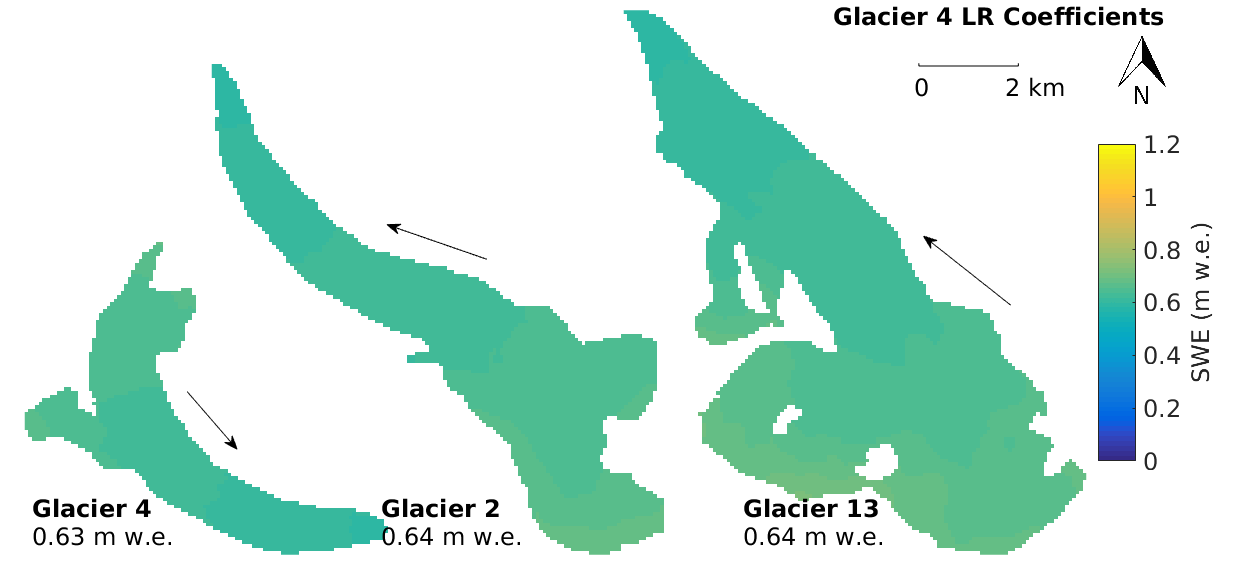
\includegraphics[width =0.9\textwidth]{MapTransferabilityG4Coeffs.png}\\
	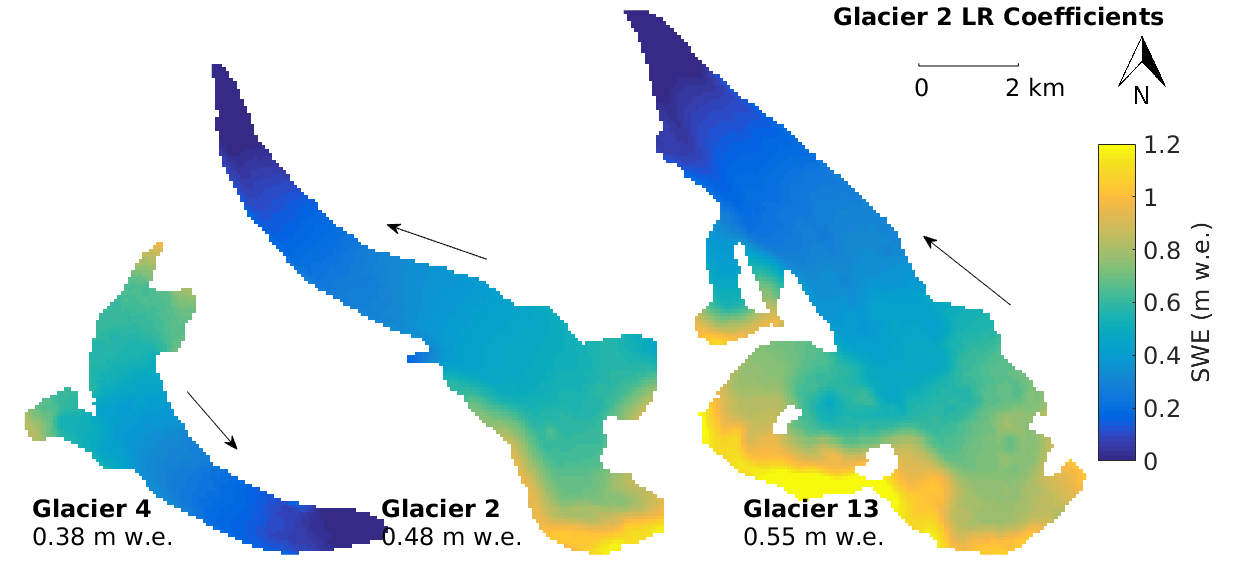
\includegraphics[width =0.9\textwidth]{MapTransferabilityG2Coeffs.png}\\
	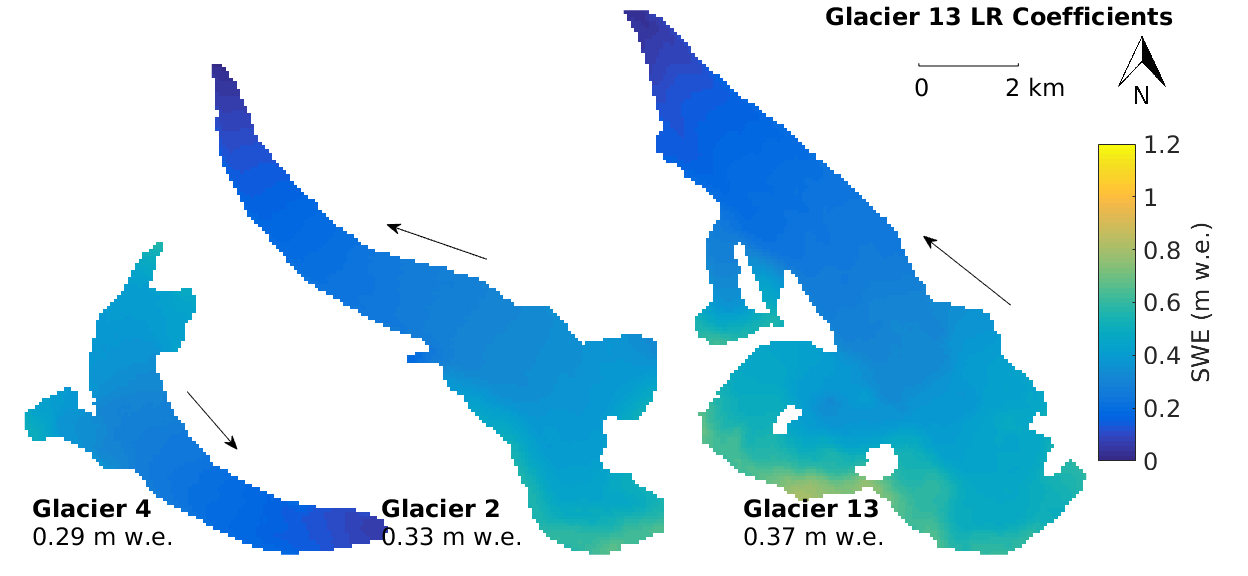
\includegraphics[width =0.9\textwidth]{MapTransferabilityG13Coeffs.png}\\
	\caption{Transfer of LR coefficients to estimate distributed winter surface mass balance (WSMB) on study glaciers. WSMB found using Glacier 4 (top), Glacier 2 (middle) and Glacier 13 (bottom) regression coefficients.  \topomap}
	\label{fig:MapTransferabilityS4}
\end{figure}

%%%%%%%%%%%%%%%%%%%%%

\end{document} 